%%%%%%%%%%%%%%%%%%%%%%%%%%%%%%%%%%%%%%%%%%%%%%%%%%%
%
%  New template code for TAMU Theses and Dissertations starting Fall 2016.
%
%
%  Original Author: Sean Zachary Roberson
%  This version adapted for URS by Parasol lab.
%  Adapted from version 3.16.10, which was last updated on 9/29/2016.
%  URS adaptation last updated 1/9/2017.
%
%%%%%%%%%%%%%%%%%%%%%%%%%%%%%%%%%%%%%%%%%%%%%%%%%%%
%%%%%%%%%%%%%%%%%%%%%%%%%%%%%%%%%%%%%%%%%%%%%%%%%%%%%%%%%%%%%%%%%%%%%%
%%                           SECTION I
%%%%%%%%%%%%%%%%%%%%%%%%%%%%%%%%%%%%%%%%%%%%%%%%%%%%%%%%%%%%%%%%%%%%%


\pagestyle{plain} % No headers, just page numbers
%\pagenumbering{arabic} % Arabic numerals
%\setcounter{page}{1}

\chapter{INTRODUCTION}

\indent The number of options people have access to is exponentially growing: millions of songs are available on Spotify, thousands of shows and movies are streamable online, and hundreds of restaurants are nearby. Due to the massive scale of the Internet, modern society provides people with a plethora of options to choose from. In the past, people shopped at physical stores, which are limited by the size of the store. By contrast, the Internet enables access to seemingly endless resources online. Amazon, for example, has an enormous collection of products but cannot display every product to every user. Due to the increase in information availability, the problem of displaying specific information to certain users arose. This gave way to information filtering systems and, more specifically, recommender systems.

For many companies, such as Amazon, Netflix, and Spotify, recommender systems drive further engagement and revenue by delivering value through a scalable way of personalizing content for their users. Modern recommender systems follow different paradigms for recommendation such as collaborative filtering, content-based recommendations, social/demographic recommendations, and contextual recommendations. Collaborative filtering compares the preferences of different users to generate predictions for users with similar preferences. Content-based recommendation leverages user preferences and domain-specific item content to generate new recommendations. Social and demographic recommendation utilizes preferences of friends, friends of friends, and demographics of similar people to suggest items. Furthermore, contextual recommendation provides recommendations based on the user's current context. For example, if a user is searching for a new car, car advertisements would be displayed and recommended as contextual recommendations.

% These paradigms typically focus on helping users discover similar items. Instead, we are interested in uncovering compatible items. For example, if a user purchases an iPhone 4, current recommender systems will recommend other similar iPhones. However, is there a way to recommend compatible iPhone 4 cases, chargers, or headphones? Although these items are not directly similar to an iPhone 4, these items should be considered equally as important to the end user since they are additional accessories that may be needed for the device and its functions.

These paradigms typically focus on helping users discover similar items. Modern recommender systems identify and understand the relationships between the items they recommend. In order to build a recommender system, a key component is that the system must have a clear definition on the relationships of items that are similar, substitutes, or complementary to develop a system that can understand a user`s intentions and recommend items \cite{linden-smith-york}.

To identify the relationships between items, this would require defining an appropriate distance or similarity measure between items or learning from training data to develop a model. Providing some metric to measure between similar items is suitable for determining an equivalence relation between items. This is to ensure that we recommend items that are considered substitutes to that item. However, a distance or similarity measure will propose issues where the compatibility between items is being considered. For example, two phone cases are similar in that they provide protection for a device and composition material, but they can be entirely different due to the devices they protect.

\section{Current Recommender Systems}
Currently, other research and industry has been aimed toward analyzing the compatibility relationships between products based on their visual appearance, textual descriptions, and ratings \cite{mcauley-pandey-leskovec, mcauley-targett-shi-hengel, menon-elkan}. Other research has used large data sets for training and provides complex models, but they follow the standard paradigm for machine learning and metric generation:

\begin{itemize}
    \item Collect a large dataset of related and unrelated items.
    \item Create a similarity function to provide distance or similarity constant.
    \item Train the function to determine related items are more similar than non-related.
\end{itemize}

These models provide a significant amount of information for distinguishing items that are similar and can range from topics of electronics to people \cite{dersaul}. The metric learning model is very flexible and powerful. However, it can ignore the details where compatibility should be considered. The current models themselves are not perfect and subject to limitations:

\begin{itemize}
    \item Similarity is either defined through an explicit category tree (e.g. `find the case nearest to this phone') and this subjects the model to noise and deficiencies in defined relations. Our model and algorithms would aim to solve this by performing recommendations without dependence on explicit relationship information.
    \item Model approaches are too strict in recommending different items. For example, an item cannot be compatible with itself or do not generate a diverse set of recommendations, such as recommending a similar product from a different brand. By analyzing the compatibility and relationships between products in a new and creative way, we can handle these issues.
\end{itemize}

Figure 1.1 describes an example of what `compatible' items would be recommended to the user given a set of queried products with a type of metric learning model: logistic regression. Logistic regression can be defined as follows.

\subsection{Logistic Regression}
Suppose $\mathbf{f}_i$ is the features that we get from product $i$ (which can be the concatenation of product image features, description features, and ratings). If $p$ is the probability that the two products are compatible, then

$$
logit(p) = b_0 + \beta \times \mathbf{X}_{ij}
$$

where $\mathbf{X}_{ij} = |\mathbf{f}_i - \mathbf{f}_j|$. 

\begin{figure}[h!]
\centering
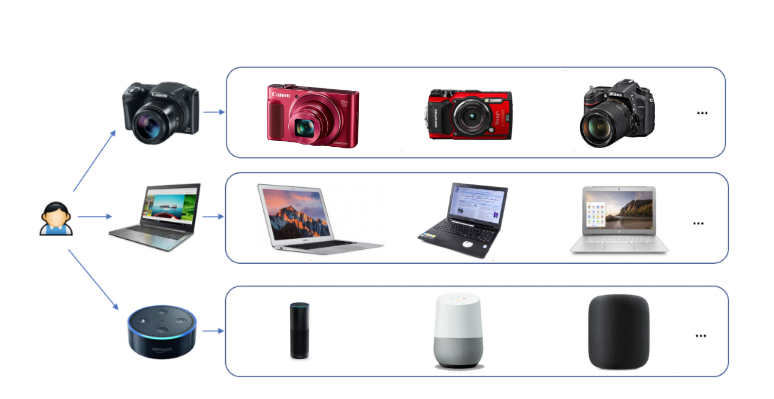
\includegraphics[scale=0.5]{data/LogisticRegression.png}
\caption{Diagram of the logistic regression model recommendations.}
\end{figure}

\section{Compatibility Recommender System}
In contrast, we are focused on discovering complementary items. For example, if a user purchases an iPhone 4, current recommender systems will recommend other similar iPhones. However, in many cases, recommending complementary items such as cases, chargers, or headphones is more relevant. Although these items are not directly similar to an iPhone 4, these items should be considered equally as important to the end user since they are additional accessories that may be needed for the device and its functions. Figure 1.2 shows an example of the compatible recommendations recommended from our compatibility classification model given the same set of queried products. 

\begin{figure}[h!]
\centering
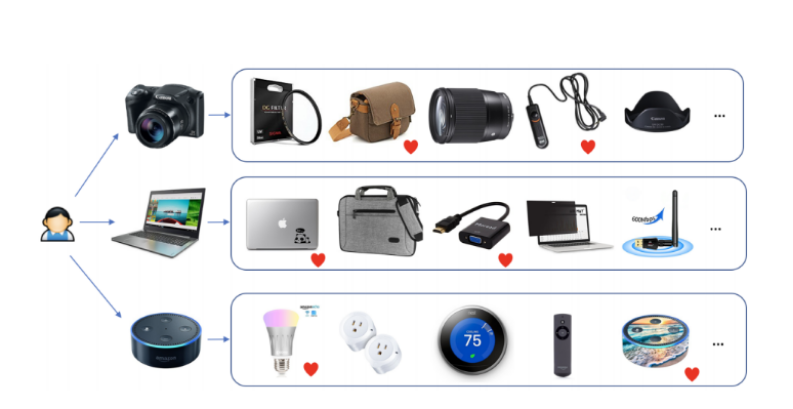
\includegraphics[scale=0.5]{data/CompatibilityModel.png}
\caption{Diagram of the compatibility model recommendations.}
\end{figure}

% For two items to be compatible, such as a phone and a charger or a dress and shoes, they must be similar in some ways but systematically different in others. Because compatibility is a human notion that is difficult to capture through the analysis of similar item relationships, compatibility of products is usually defined manually through expert individuals or assumed through the co-purchasing habits of customers. For example, if a customer buys an iPhone and then buys an iPhone charger, it is assumed that this iPhone and this iPhone charger are compatible. However, how about if this same customer purchases an iPhone and then a t-shirt? Are these now considered compatible? Therefore, it is not clear how to identify compatible items, especially for large and varied products sets. In a sample of 500,000 products in Electronics on Amazon, only 20\% explicitly mention “compatibility” with another product.2 Another challenging aspect is finding the number of items that are actually compatible with the queried product amongst a huge dataset. This could be less than 1\%! Thus, our research focuses on defining a new definition of compatibility in item recommender systems to provide scalable, improved item recommendation. 

For two items to be compatible, such as a phone and a charger or a dress and shoes, they must be similar in some ways but systematically different in others. Because compatibility is a human notion that is difficult to capture through the analysis of similar item relationships, compatibility of products is usually defined manually through expert individuals or assumed through the co-purchasing habits of customers, like on Amazon. In a sample of 500,000 products in Electronics on Amazon, only 20\% explicitly mention "compatibility" with another product, and therefore, assuming compatibility through co-purchasing habits can be very effective on a large scale but can be very prone to noise. For example, if a customer purchases an iPhone and an iPhone charger together, it is assumed that the iPhone and iPhone charger are compatible. However, the issue arises when a customer purchases two entirely unrelated products such as an iPhone and a t-shirt. The recommender system will now assume these two items are compatible when in reality they are not. Therefore, it is not clear how to correctly identify compatible items, especially for large and varied product sets. Another challenging aspect is finding the number of items that are compatible with the queried product among a huge dataset. Due to the large product data, randomly selecting an item has a less than 1\% chance of being compatible with the desired item. Thus, our research focuses on defining a new definition of compatibility in item recommender systems to provide scalable, improved item recommendation.

% In a sample of 500,000 products in Electronics on Amazon only 20\% explicitly mention "compatibility" with another product. Another challenging aspect is finding the number of items that are actually compatible with the queried product among a huge dataset. This could be less than 1\%! Thus, our research focuses on defining a new definition of compatibility in item recommender systems to provide scalable, improved item recommendation.

While using our improved item recommendation model, not only do customers have a more personalized space to do their shopping, but sellers also have a higher chance of being recommended to users, which may increase their revenue and product views. This is phenomenon is otherwise known as the cold-start problem. The cold-start problem is the issue where new products that are placed on the marketplace do not get as much attention as the older, more reviewed products. This is because of the co-purchasing effect, where items on Amazon are recommended based on customers and their buying techniques. Because these items are new and have not been bought with other items, the chances of these items making it into recommendation systems are very slim. However, our recommender system will solve this issue by not deriving compatibility from co-purchasing items but rather from the analysis of the product and its relation to other products in more concrete ways.

% In our research, we will propose new models and algorithms to identify the relationships between items in product recommendation settings. The new models and algorithms will utilize our definition of compatibility to create a more relevant and accurate way to recommend items.

